\documentclass[11pt,a4paper,oneside]{article}

%------------------------------------------------------------
% PACKAGES
%------------------------------------------------------------
\usepackage[top=25mm, bottom=25mm, left=25mm, right=25mm,
            headheight=15pt]{geometry}
\usepackage[spanish,es-noshorthands]{babel}
\usepackage{setspace}
\usepackage{mathptmx}
\usepackage[T1]{fontenc}
\usepackage[utf8]{inputenc}
\usepackage{graphicx}
\usepackage{float}
\usepackage{booktabs}
\usepackage{tabularx}
\usepackage{array}
\usepackage{amsmath}
\usepackage{amssymb}
\usepackage{caption}
\usepackage{xcolor}
\usepackage{hyperref}
\usepackage{fancyhdr}
\usepackage{titlesec}
\usepackage{enumitem}
\usepackage{microtype}
\usepackage{colortbl}
\usepackage{placeins}
\usepackage{csquotes}
\usepackage[backend=biber,style=ieee]{biblatex}

\addbibresource{references.bib}

\addto\captionsspanish{\renewcommand{\tablename}{Tabla}}

%------------------------------------------------------------
% SHORT TITLES FOR HEADER
%------------------------------------------------------------
\def\ProjectTitleShort{Reproducción de RBlockSim}
\def\DeptShort{Escuela Profesional de Ciencia de la Computación}

%------------------------------------------------------------
% COLOURS
%------------------------------------------------------------
\definecolor{dtunavy}{RGB}{0, 32, 91}
\definecolor{tablehead}{RGB}{0, 32, 91}

\hypersetup{
  colorlinks=true,
  linkcolor=dtunavy,
  citecolor=dtunavy,
  urlcolor=dtunavy,
  pdftitle={Reproducción de RBlockSim: Simulación Paralela y Distribuida para Blockchain},
}

%------------------------------------------------------------
% LINE SPACING
%------------------------------------------------------------
\setstretch{1.15}
\raggedbottom

%------------------------------------------------------------
% SECTION FORMAT
%------------------------------------------------------------
\titleformat{\section}
  {\bfseries\Large}
  {\thesection}
  {1em}
  {}

\titleformat{\subsection}
  {\bfseries\normalsize}
  {\thesubsection}
  {1em}
  {}

\titlespacing*{\section}
  {0pt}
  {14pt}
  {8pt}

\titlespacing*{\subsection}
  {0pt}
  {10pt}
  {4pt}

%------------------------------------------------------------
% CAPTION STYLE
%------------------------------------------------------------
\captionsetup[table]{position=above, labelfont=bf, font=small}
\captionsetup[figure]{position=below, labelfont=bf, font=small}

%------------------------------------------------------------
% HEADER/FOOTER
%------------------------------------------------------------
\pagestyle{fancy}
\fancyhf{}
\fancyhead[R]{\small\textit{\ProjectTitleShort}}
\fancyhead[L]{\small\textit{\DeptShort, UNSA}}
\fancyfoot[C]{\thepage}
\renewcommand{\headrulewidth}{0.4pt}

%============================================================
\begin{document}
%============================================================

\pagenumbering{roman}
\pagestyle{empty}

%============================================================
%  TITLE PAGE
%============================================================
\def\myauthor{Alva Cornejo, Jose Javier}
\def\myteacher{Alvaro Henry Mamani Aliaga}
\def\mytitle{Reproducción de RBlockSim: Simulación Paralela y Distribuida para Blockchain}
\def\mycourse{COMPUTACIÓN PARALELA Y DISTRIBUIDA}
\def\myCUI{20230573}

\newgeometry{margin=1.25in}
\begin{titlepage}
	\centering
	{\LARGE\bfseries UNIVERSIDAD NACIONAL DE SAN AGUSTÍN \par}
	{\large Facultad de Ingeniería de Producción y Servicios\\
	Escuela Profesional de Ciencia de la Computación}\\\vspace{0.4cm}
	
\includegraphics[width=0.52\textwidth]{unsa}\\\vspace{0.2cm}
    \Large\bf\mycourse\\\vspace{0.3cm}

	{\LARGE\bfseries \mytitle\par}
	\vspace{0.25cm}
	{\large\bfseries Informe integrado de resultados\par}
	\vspace{0.7cm}
    {\large {Docente:} \textsc{\myteacher}}\\\vspace{0.35cm}
	{\large {Integrantes:} \par}
	{\normalsize \textsc{Alva Cornejo, Jose Javier} \; (\myCUI)\\
	\textsc{Carpio Paiva, Cesar Gonzalo}\\
	\textsc{Palomino Rivadeneyra, Misael}\\
	\textsc{Zapana Pariapaza, Gonzalo Rodrigo}\par}

	\vfill

	{\large Arequipa -- Perú \par \today \par}
\end{titlepage}

\restoregeometry

%============================================================
%  MAIN TEXT
%============================================================
\cleardoublepage
\pagenumbering{arabic}
\setcounter{page}{1}

%============================================================
%  RESUMEN
%============================================================
\section*{Resumen}

Este informe sintetiza la reproducción experimental de \emph{RBlockSim}, un simulador paralelo y distribuido de redes blockchain construido sobre el runtime ROOT-Sim. Se utilizan exclusivamente los resultados de la ejecución \texttt{\_1}: las figuras regeneradas a partir de los archivos de salida y un conjunto de indicadores calculados directamente sobre los datos crudos. La validación estadística del modelo de Proof of Work se reproduce con alta fidelidad ($R^2 \ge 0.9969$ y MAE $\le 0.0127$). Los ataques del 51\,\% y de minería egoísta mantienen las tendencias del artículo, con errores medios absolutos de 0.020--0.031 y de 0.024--0.103 según la profundidad. El uso de memoria es consistente en orden de magnitud: 3.5--5.0\,GB para 10\,000 nodos y 16.6--24.9\,GB para 50\,000. El rendimiento solo pudo evaluarse con 1, 4 y 8 hilos; mejora en redes grandes (hasta $2.02\times$) pero se degrada en redes pequeñas. La reproducibilidad funcional y estadística es alta; la de rendimiento queda limitada por el hardware y por la ausencia de repeticiones.

%============================================================
%  1. INTRODUCCIÓN
%============================================================
\section{Introducción}

\subsection{Contexto y objetivo}

Las redes blockchain registran transacciones de forma descentralizada y dependen de la interacción entre nodos, bloques, retardos de red y posibles comportamientos adversarios \cite{nakamoto2008bitcoin}. Evaluar su rendimiento y su seguridad a escala real es costoso, por lo que la simulación se utiliza para estudiar propiedades emergentes en un entorno controlado. \emph{RBlockSim} \cite{pimpini2025rblocksim} combina un modelo modular de blockchain con el runtime de simulación de eventos discretos optimista ROOT-Sim \cite{pellegrini2012rootsim}, y permite distribuir los procesos lógicos entre varios núcleos \cite{fujimoto1990pdes}.

Este trabajo reproduce los resultados del artículo de Pimpini y Pellegrini presentado en SIGSIM-PADS 2025. El objetivo de este informe es responder tres preguntas concretas: si el modelo estadístico de Proof of Work se reproduce, si los ataques del 51\,\% y de minería egoísta mantienen las tendencias publicadas, y si el rendimiento y el uso de memoria son comparables. A diferencia de un informe exhaustivo, aquí se integran la evidencia visual de las figuras con unos pocos indicadores calculados sobre los datos crudos, sin desarrollar el marco teórico ni repetir todas las tablas de comparación.

\subsection{Alcance y organización}

La reproducción cubrió la validación estadística (Figura~3 del artículo), los ataques (Figuras~4 y~5), el tiempo de ejecución (Figura~6), la memoria máxima (Figura~7) y la evolución agregada de memoria (Figura~8 del artículo). Se utilizó una máquina con 12 vCPU y 31\,GiB de RAM, y se ejecutó una sola iteración por configuración. Estas condiciones limitaron el número de hilos y el tamaño máximo de red, como se detalla en la Sección~\ref{sec:metodologia}. La Sección~\ref{sec:resultados} presenta los resultados; la Sección~\ref{sec:comparacion} incluye la comparación visual con las figuras originales, la síntesis y las limitaciones; la Sección~\ref{sec:conclusiones} cierra con las conclusiones.

%============================================================
%  2. METODOLOGÍA
%============================================================
\section{Metodología}
\label{sec:metodologia}

\subsection{Artefacto y datos utilizados}

La reproducción se realizó sobre el repositorio oficial \texttt{RBlockSim\_Reproducibility}, disponible en \url{https://github.com/AdrianoPi/RBlockSim_Reproducibility}. El artefacto está containerizado con Docker y organiza la campaña en tres bloques: ataques, rendimiento y evolución de memoria (Figura~8 del artículo). El script \texttt{reproduce.sh} construye la imagen y ejecuta \texttt{entrypoint.py}, que lanza las simulaciones y genera las figuras.

Se utilizaron exclusivamente los resultados de la ejecución \texttt{\_1}: las figuras de \path{reproduced/plots/plots_1} y los archivos crudos de ataques, rendimiento y Figura~8 del artículo. La carpeta \texttt{\_0} se descartó por corresponder a una ejecución incompleta. Para el análisis numérico se leyeron los archivos \texttt{out\_*.txt} (tiempo de simulación), los JSON de estadísticas por nodo (bloques y ataques), los JSON de picos de RAM y los metadatos con el historial de memoria.

\subsection{Configuración y entorno}

La Tabla~\ref{tab:config} resume la campaña y el entorno. Los ataques usaron 8 hilos, un intervalo de bloque de 600\,s y una duración simulada de 24\,h. El rendimiento se evaluó con intervalos de 13\,s y 600\,s; de los ocho números de hilos previstos, solo 1, 4 y 8 finalizaron correctamente. La Figura~8 del artículo se reprodujo con 1\,000, 10\,000 y 50\,000 nodos. La red de 50\,000 nodos sustituyó a la de 100\,000 nodos del artículo por limitaciones de memoria y tiempo.

\begin{table}[htbp]
\caption{Configuración de la campaña y entorno de ejecución.}
\label{tab:config}
\centering
\small
\renewcommand{\arraystretch}{1.12}
\begin{tabularx}{\textwidth}{>{\raggedright\arraybackslash}p{0.30\textwidth}X}
\toprule
\rowcolor{tablehead}
\textcolor{white}{\textbf{Aspecto}} &
\textcolor{white}{\textbf{Valor}} \\
\midrule
Modo de reproducción & \texttt{all} (ataques, rendimiento y RAM agregada) \\
Ataques & 100, 1\,000 y 10\,000 nodos; 8 hilos; BI de 600\,s; 24\,h; $h=0.01$--$0.99$ \\
Rendimiento & 100, 1\,000, 10\,000 y 50\,000 nodos; BI de 13\,s y 600\,s; 1, 4 y 8 hilos válidos \\
Figura~8 del artículo & 1\,000, 10\,000 y 50\,000 nodos; 8 hilos; BI de 600\,s \\
Iteraciones & 1 por configuración \\
Equipo de reproducción & Intel Core i7-10850H, 6 núcleos / 12 hilos, 31\,GiB de RAM \\
Equipo del artículo & 2 $\times$ Intel Xeon E5-2696 v4, 44 núcleos / 88 hilos, 256\,GB de RAM \\
\bottomrule
\end{tabularx}
\end{table}

Los ataques se ejecutaron solo a 100, 1\,000 y 10\,000 nodos; no se realizaron ataques a 50\,000. La red de 50\,000 se usa únicamente en los experimentos de rendimiento y en la Figura~8 del artículo.

\subsection{Métricas y depuración de datos}

Para la validación estadística se comparó la tasa de minería observada $y_i$ con la tasa de hash esperada $x_i$ mediante el coeficiente de determinación $R^2$, el error absoluto medio $\mathrm{MAE}=n^{-1}\sum_i |y_i-x_i|$ y la raíz del error cuadrático medio. Para los ataques se usó el MAE respecto de la diagonal $y=x$ y la tasa de éxito de la minería egoísta. Para el rendimiento se calculó el speedup $S(p)=T(1)/T(p)$, donde $T(p)$ es el tiempo con $p$ hilos.

Las ejecuciones con 16, 22, 44, 66 y 88 hilos no iniciaron porque la máquina solo dispone de 12 unidades de cómputo; ROOT-Sim reportó \texttt{Demanding N cores, which is more than available (12)}. Esos registros se excluyeron, junto con los picos de RAM residuales del orden de $10^{-3}$\,GB. El trazador original no filtra las ejecuciones fallidas y las dibuja como cero, por lo que las Figuras~5 y~6 se regeneraron usando solo las configuraciones válidas. Las Figuras~1--4 se regeneraron a partir de los JSON procesados, con etiquetas en español y un estilo uniforme.

%============================================================
%  3. RESULTADOS
%============================================================
\section{Resultados}
\label{sec:resultados}

\subsection{Validación estadística}

La Figura~\ref{fig:validacion} compara la tasa de minería observada con la tasa de hash asignada en las tres redes. En los tres casos la curva sigue de cerca la diagonal. La Tabla~\ref{tab:validacion} cuantifica el ajuste: $R^2$ entre 0.9969 y 0.9989, MAE entre 0.0086 y 0.0127 y RMSE entre 0.0095 y 0.0159. El mejor ajuste corresponde a 1\,000 nodos y el mayor error a 10\,000 nodos.

\begin{figure}[tbp]
  \centering
  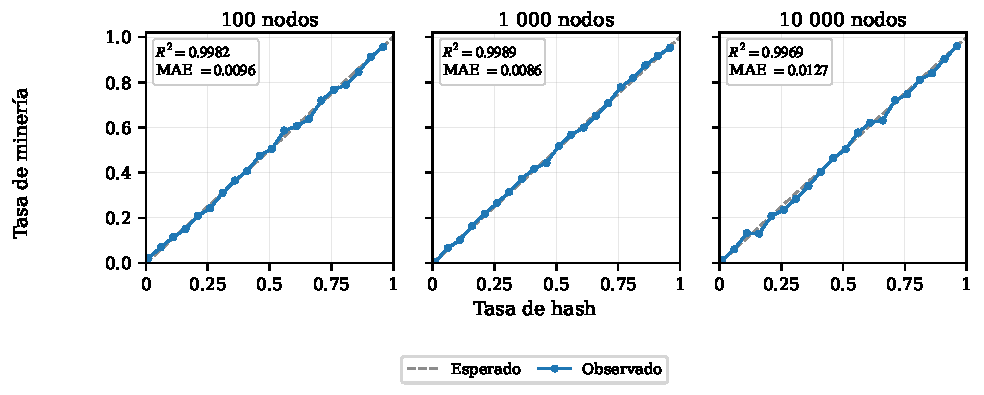
\includegraphics[width=\textwidth]{figures/fig_validacion.pdf}
  \caption{Validación estadística del modelo de Proof of Work (equivalente a la Figura~3 del artículo). La línea gris punteada es la relación esperada $y=x$; la línea azul es la tasa de minería observada. Los paneles corresponden a 100, 1\,000 y 10\,000 nodos.}
  \label{fig:validacion}
\end{figure}

\begin{table}[htbp]
\caption{Métricas de validación estadística.}
\label{tab:validacion}
\centering
\small
\renewcommand{\arraystretch}{1.12}
\begin{tabular}{lccc}
\toprule
\rowcolor{tablehead}
\textcolor{white}{\textbf{Nodos}} &
\textcolor{white}{\textbf{$R^2$}} &
\textcolor{white}{\textbf{MAE}} &
\textcolor{white}{\textbf{RMSE}} \\
\midrule
100    & 0.9982 & 0.0096 & 0.0122 \\
1\,000 & 0.9989 & 0.0086 & 0.0095 \\
10\,000 & 0.9969 & 0.0127 & 0.0159 \\
\bottomrule
\end{tabular}
\end{table}

Las diferencias son compatibles con una sola realización por configuración y con el número finito de bloques. Con un intervalo de 600\,s y una duración de 24\,h se minan del orden de 145 bloques por ejecución; con 13\,s, alrededor de 6\,650. La proximidad a la diagonal confirma que el generador de bloques respeta la proporcionalidad entre potencia de hash y tasa de minería.

\FloatBarrier
\subsection{Ataques del \texorpdfstring{51\,\%}{51\%} y de minería egoísta}

La Figura~\ref{fig:51} muestra el ataque del 51\,\%. Las curvas de ambas tolerancias se mantienen cerca de la diagonal: el MAE se sitúa entre 0.020 y 0.031 y el error máximo no supera 0.10. No se observa una aceptación desproporcionada de bloques del atacante ni una diferencia relevante entre tolerancias.

\begin{figure}[tbp]
  \centering
  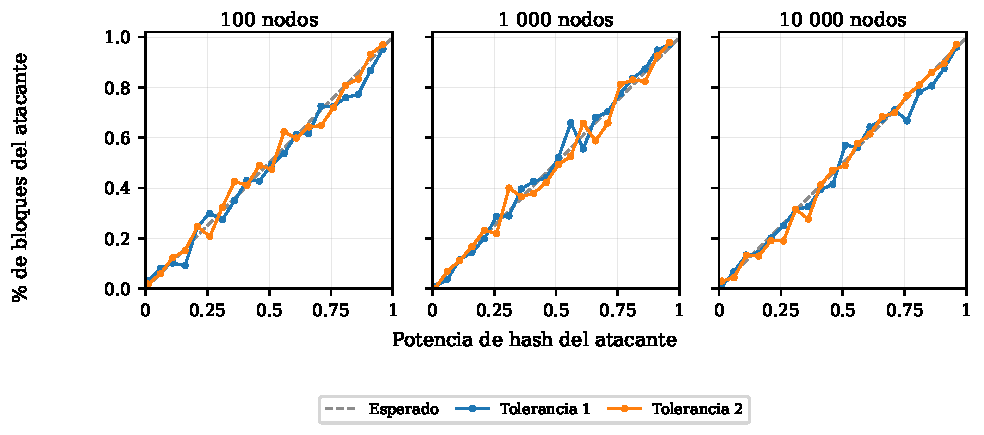
\includegraphics[width=\textwidth]{figures/fig_51.pdf}
  \caption{Ataque del 51\,\% (equivalente a las Figuras~4a--4c del artículo). Porcentaje de bloques del atacante en la cadena principal frente a su potencia de hash, para las tolerancias 1 y 2. La línea gris punteada es la relación esperada $y=x$. Los paneles corresponden a 100, 1\,000 y 10\,000 nodos.}
  \label{fig:51}
\end{figure}

Las Figuras~\ref{fig:selfish} y~\ref{fig:success} resumen la minería egoísta \cite{eyal2014majority}. El porcentaje de bloques comprometidos crece con la potencia de hash y la tasa de éxito se satura cerca de 1.0 para $h>0.8$. La profundidad 3 se separa de la diagonal en potencias bajas y medias: el atacante compromete menos bloques de los que le corresponderían por su potencia. El MAE es 0.024--0.032 con profundidad 1, 0.063--0.081 con profundidad 2 y 0.084--0.103 con profundidad 3.

\begin{figure}[tbp]
  \centering
  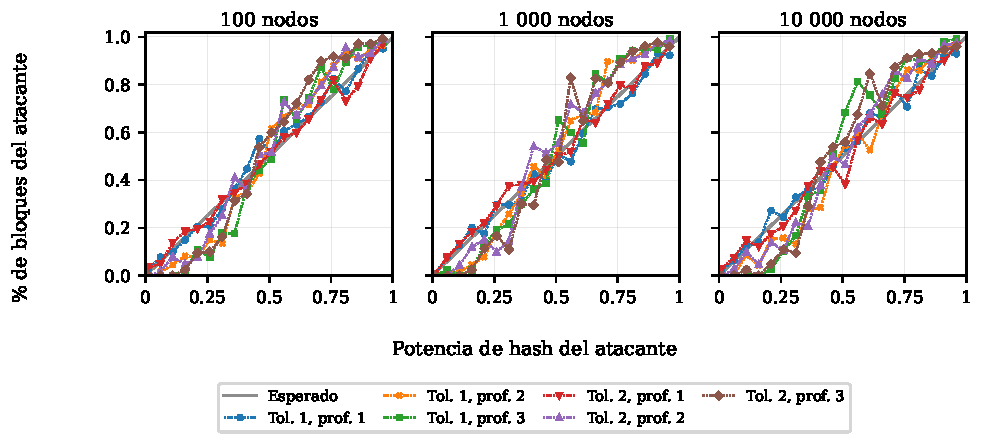
\includegraphics[width=\textwidth]{figures/fig_selfish_committed.pdf}
  \caption{Minería egoísta: porcentaje de bloques del atacante en la cadena principal (equivalente a las Figuras~4d--4f del artículo). Se muestran dos tolerancias y tres profundidades. La línea gris es la relación esperada $y=x$. Los paneles corresponden a 100, 1\,000 y 10\,000 nodos.}
  \label{fig:selfish}
\end{figure}

\begin{figure}[tbp]
  \centering
  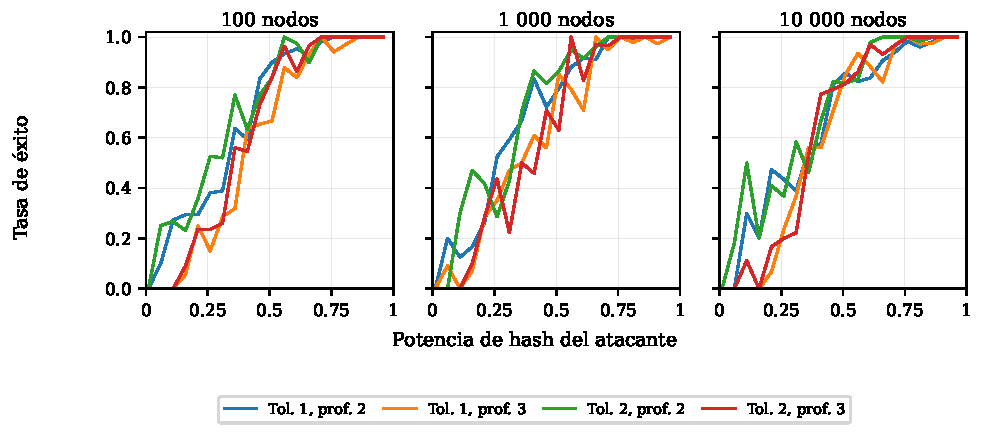
\includegraphics[width=\textwidth]{figures/fig_selfish_success.pdf}
  \caption{Tasa de éxito de la minería egoísta (equivalente a la Figura~5 del artículo). Los paneles corresponden a 100, 1\,000 y 10\,000 nodos; las curvas corresponden a las combinaciones de tolerancia y profundidad indicadas.}
  \label{fig:success}
\end{figure}

En potencias bajas ($h\approx 0.26$--$0.36$) la tasa de éxito es dispersa: 0.15--0.59. En $h\approx 0.51$ se sitúa entre 0.63 y 0.90, y para $h>0.75$ alcanza 0.94--1.00. La dispersión es mayor que en el artículo porque la reproducción usa una sola iteración por configuración, mientras que el artículo promedia cinco ejecuciones.

\FloatBarrier
\subsection{Rendimiento}

La Figura~\ref{fig:performance} presenta los tiempos de ejecución para los únicos números de hilos válidos: 1, 4 y 8. La Tabla~\ref{tab:performance} contiene los valores numéricos, los speedups y la RAM máxima. En las redes de 100 y 1\,000 nodos el tiempo aumenta al pasar de 1 a 4 y a 8 hilos. Para 100 nodos y BI de 13\,s, el tiempo pasa de 1.40\,s a 58.84\,s y 496.97\,s ($S(8)=0.003$); para 1\,000 nodos, de 15.87\,s a 31.18\,s y 113.96\,s ($S(8)=0.14$).

\begin{figure}[t]
  \centering
  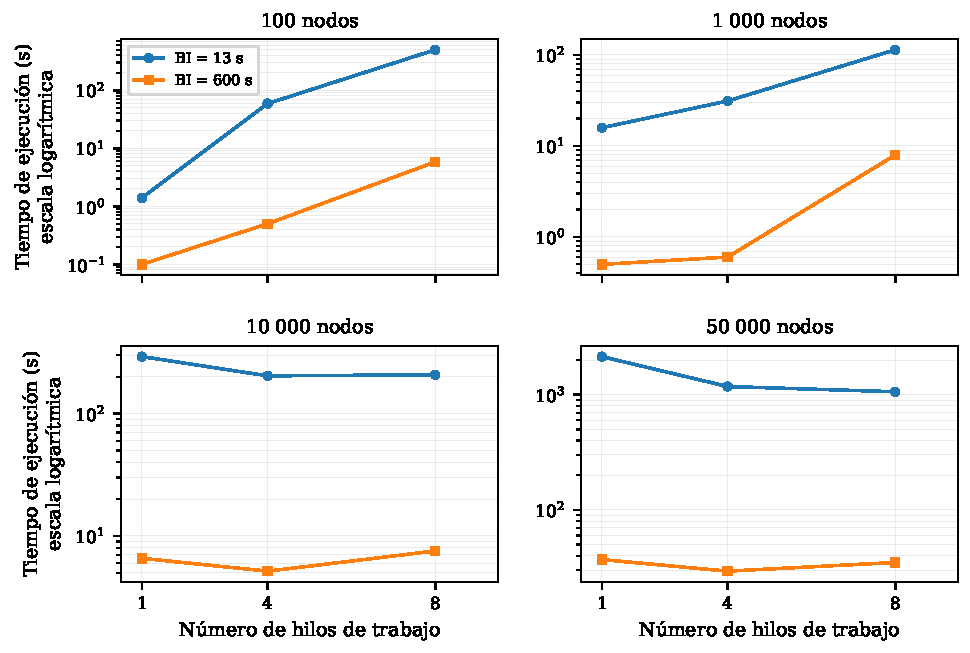
\includegraphics[width=\textwidth]{figures/fig_performance.pdf}
  \caption{Tiempos de ejecución reproducidos para 1, 4 y 8 hilos de trabajo. Solo se muestran las configuraciones que finalizaron correctamente en la máquina de 12 vCPU. Los paneles corresponden a 100, 1\,000, 10\,000 y 50\,000 nodos. El eje vertical es logarítmico.}
  \label{fig:performance}
\end{figure}

\begin{table}[htbp]
\caption{Tiempos, speedups y RAM máxima reproducidos (solo configuraciones válidas). La RAM se expresa como rango entre 1, 4 y 8 hilos.}
\label{tab:performance}
\centering
\footnotesize
\setlength{\tabcolsep}{3.5pt}
\renewcommand{\arraystretch}{1.10}
\begin{tabular}{lccccccc}
\toprule
\rowcolor{tablehead}
\textcolor{white}{\textbf{Nodos}} &
\textcolor{white}{\textbf{BI (s)}} &
\textcolor{white}{\textbf{$T(1)$ (s)}} &
\textcolor{white}{\textbf{$T(4)$ (s)}} &
\textcolor{white}{\textbf{$T(8)$ (s)}} &
\textcolor{white}{\textbf{$S(4)$}} &
\textcolor{white}{\textbf{$S(8)$}} &
\textcolor{white}{\textbf{RAM (GB)}} \\
\midrule
100     & 13  & 1.40    & 58.84   & 496.97  & 0.02 & 0.003 & 0.15--0.23 \\
100     & 600 & 0.10    & 0.50    & 5.81    & 0.20 & 0.017 & 0.0004--0.105 \\
1\,000  & 13  & 15.87   & 31.18   & 113.96  & 0.51 & 0.14  & 0.64--0.71 \\
1\,000  & 600 & 0.50    & 0.60    & 7.94    & 0.83 & 0.06  & 0.001--0.606 \\
10\,000 & 13  & 292.03  & 203.33  & 207.49  & 1.44 & 1.41  & 4.89--5.03 \\
10\,000 & 600 & 6.56    & 5.15    & 7.54    & 1.27 & 0.87  & 3.47--3.56 \\
50\,000 & 13  & 2\,146.35 & 1\,179.81 & 1\,062.81 & 1.82 & 2.02 & 23.5--24.9 \\
50\,000 & 600 & 37.03   & 29.35   & 34.95   & 1.26 & 1.06  & 16.6--17.1 \\
\bottomrule
\end{tabular}
\end{table}

En 10\,000 nodos el mejor resultado se obtiene con 4 hilos ($S=1.44$ para BI de 13\,s y $S=1.27$ para 600\,s). En 50\,000 nodos se alcanza $2.02\times$ con 8 hilos para BI de 13\,s y $1.26\times$ con 4 hilos para 600\,s. Los tiempos de un hilo son mucho menores que los del artículo (15.87\,s frente a 392.06\,s en 1\,000 nodos; 292.03\,s frente a 5\,965.97\,s en 10\,000), por lo que la comparación de tiempos absolutos no es directa. Las ejecuciones con BI de 600\,s duran entre 0.1 y 37\,s; en ese rango el arranque y la variabilidad pesan más, así que las conclusiones de rendimiento se apoyan principalmente en BI de 13\,s.

\FloatBarrier
\subsection{Uso de memoria}

La Figura~\ref{fig:ram} muestra la RAM máxima reproducida. Para 10\,000 nodos se obtiene 3.5--5.0\,GB, dentro del rango aproximado de 3.4--5.9\,GB del artículo. Para 50\,000 nodos se obtiene 16.6--24.9\,GB, consistente con un crecimiento aproximadamente lineal respecto de los 35--47\,GB que el artículo reporta para 100\,000 nodos. Los valores por debajo de 0.01\,GB en 100 y 1\,000 nodos con BI de 600\,s son artefactos de ejecuciones de 0.1--0.6\,s: el muestreador de memoria no alcanza a registrar el pico real.

La Figura~\ref{fig:ram_history} muestra la evolución agregada de la memoria durante la simulación. La memoria crece rápidamente al inicio, se estabiliza y permanece acotada hasta el final. Las mesetas son aproximadamente 0.6\,GB para 1\,000 nodos, 3.6\,GB para 10\,000 y 16.6\,GB para 50\,000. La forma de las curvas coincide con la de la Figura~8 del artículo, aunque los valores absolutos son menores.

\begin{figure}[H]
  \centering
  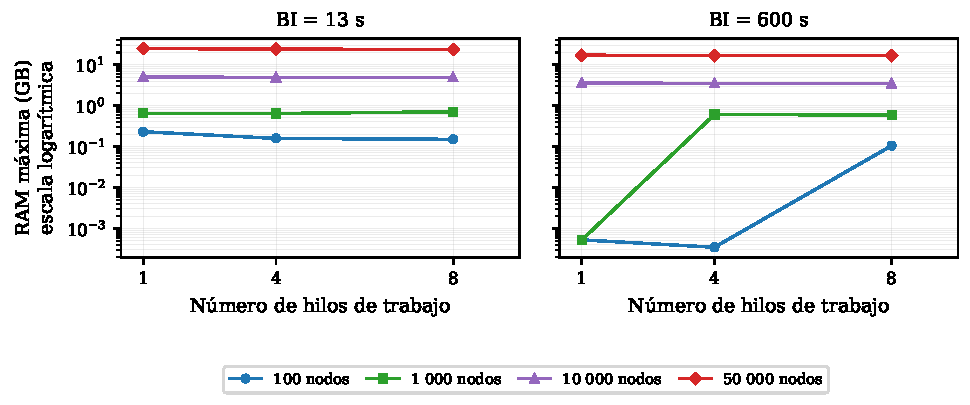
\includegraphics[width=\textwidth]{figures/fig_ram.pdf}
  \caption{RAM máxima reproducida para 1, 4 y 8 hilos. Solo se incluyen configuraciones válidas. Se usan redes de 100, 1\,000, 10\,000 y 50\,000 nodos. El eje vertical es logarítmico. Los valores inferiores a 0.01\,GB corresponden a ejecuciones muy cortas y deben interpretarse con cautela.}
  \label{fig:ram}
\end{figure}

\begin{figure}[H]
  \centering
  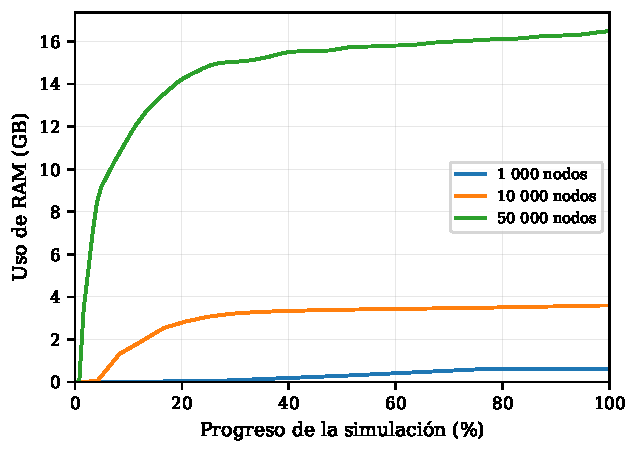
\includegraphics[width=0.72\textwidth]{figures/fig_ram_history.pdf}
  \caption{Evolución agregada del uso de RAM durante la simulación para 1\,000, 10\,000 y 50\,000 nodos (equivalente a la Figura~8 del artículo). No se ejecutaron redes de 100\,000 nodos.}
  \label{fig:ram_history}
\end{figure}

%============================================================
%  4. COMPARACIÓN Y LIMITACIONES
%============================================================
\section{Comparación con el artículo y limitaciones}
\label{sec:comparacion}

\subsection{Comparación visual con el artículo}
\label{sec:comparacion-visual}

Las Figuras~\ref{fig:cmp-validacion-exito} a~\ref{fig:cmp-memoria} confrontan las figuras originales del artículo con las reproducciones. Las originales se extrajeron de \cite{pimpini2025rblocksim}; las reproducciones usan exclusivamente los datos de la ejecución \texttt{\_1}. La comparación no busca que cada punto coincida, sino verificar tendencias, rangos y conclusiones.

\begin{figure}[H]
  \centering
  \begin{minipage}[t]{0.43\textwidth}
    \centering
    {\small\textbf{Artículo}\par}
    \vspace{0.2em}
    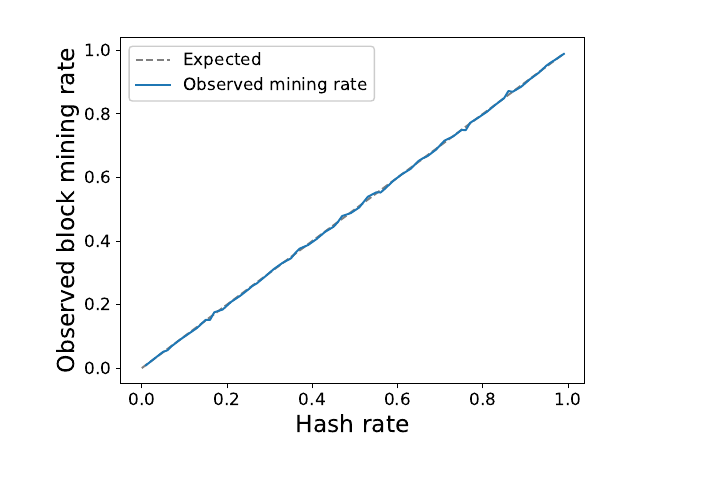
\includegraphics[width=\linewidth]{figures/paper_original/figure3_hi.png}
  \end{minipage}\hfill
  \begin{minipage}[t]{0.43\textwidth}
    \centering
    {\small\textbf{Reproducción}\par}
    \vspace{0.2em}
    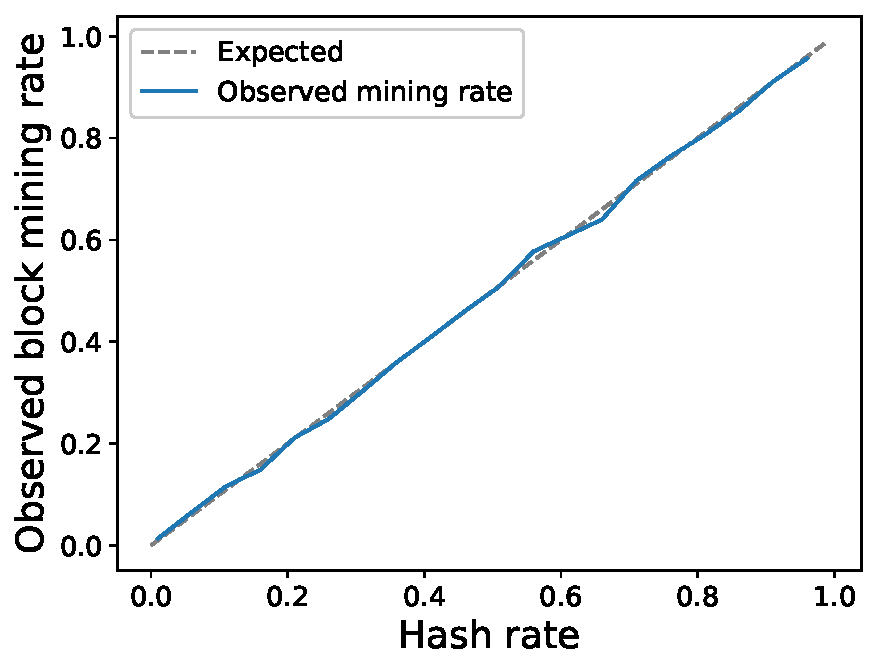
\includegraphics[width=\linewidth]{figures/Figure_3.pdf}
  \end{minipage}

  \par\vspace{0.4em}
  {\small\textbf{Artículo (Figura~5)}\par}
  \vspace{0.2em}
  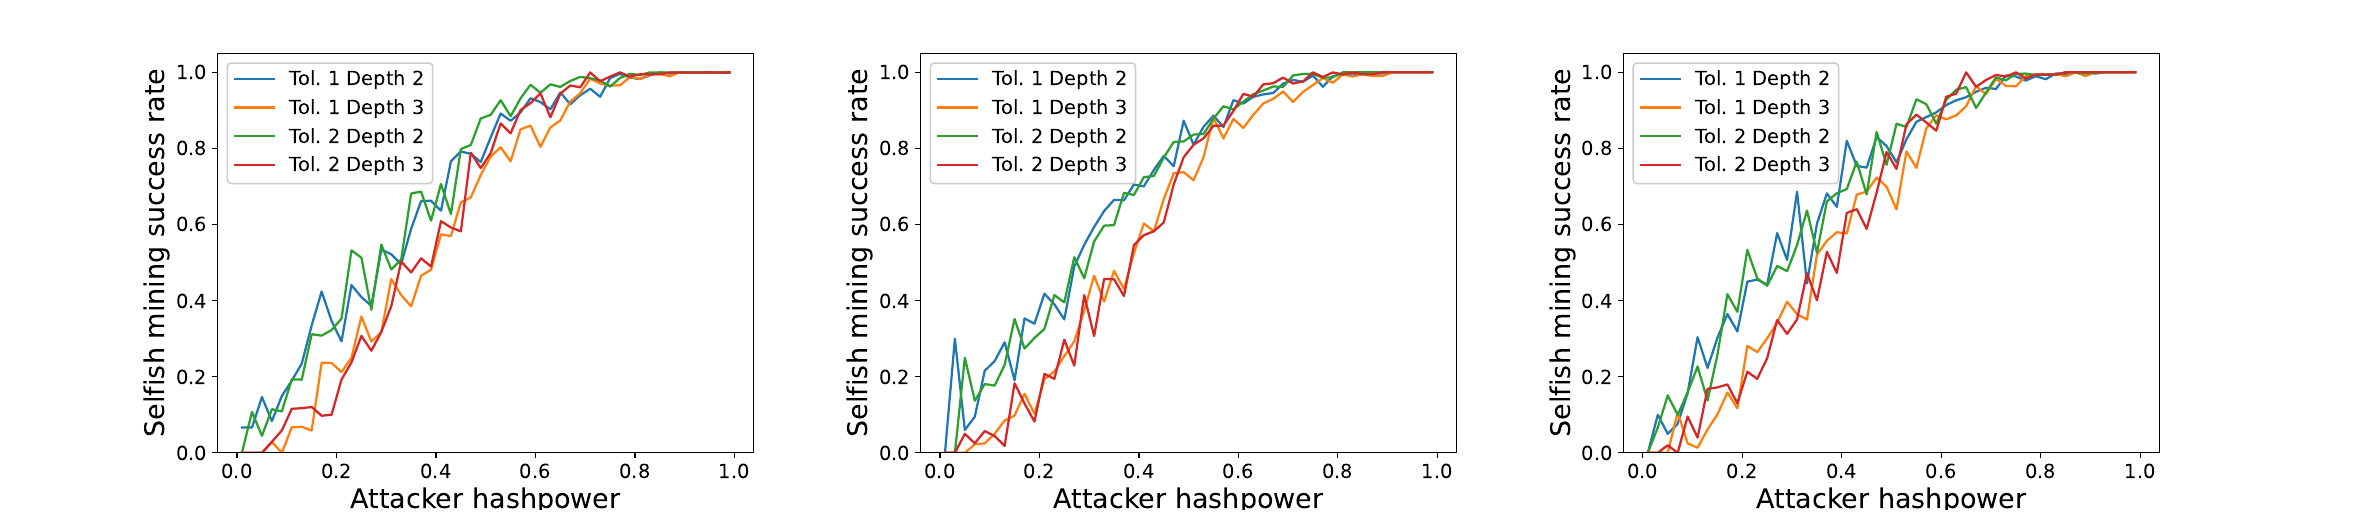
\includegraphics[width=0.90\textwidth]{figures/paper_original/figure5_hi.png}

  \par\vspace{0.2em}
  {\small\textbf{Reproducción (Figura~4)}\par}
  \vspace{0.2em}
  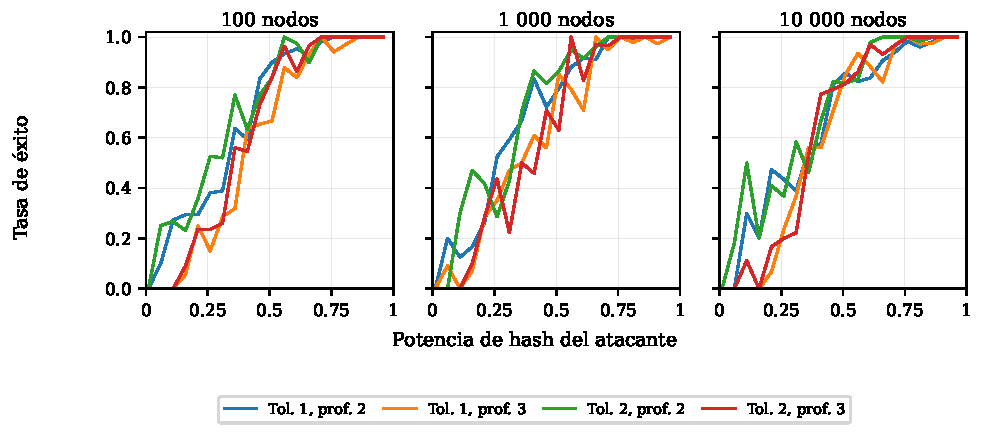
\includegraphics[width=0.90\textwidth]{figures/fig_selfish_success.pdf}
  \caption{Comparación de la validación estadística y de la tasa de éxito de la minería egoísta. Arriba: Figura~3 del artículo frente a la reproducción en un panel; el desglose por tamaño con $R^2$ y MAE está en la Figura~\ref{fig:validacion}. Abajo: Figura~5 del artículo frente a la reproducción. Las figuras originales provienen de \cite{pimpini2025rblocksim}.}
  \label{fig:cmp-validacion-exito}
\end{figure}

La validación reproduce la diagonal con $R^2 \ge 0.9969$ y MAE $\le 0.0127$. La tasa de éxito se satura para $h>0.75$; las curvas son más irregulares por usar una sola iteración.

\begin{figure}[H]
  \centering
  {\small\textbf{Artículo (Figura~4)}\par}
  \vspace{0.2em}
  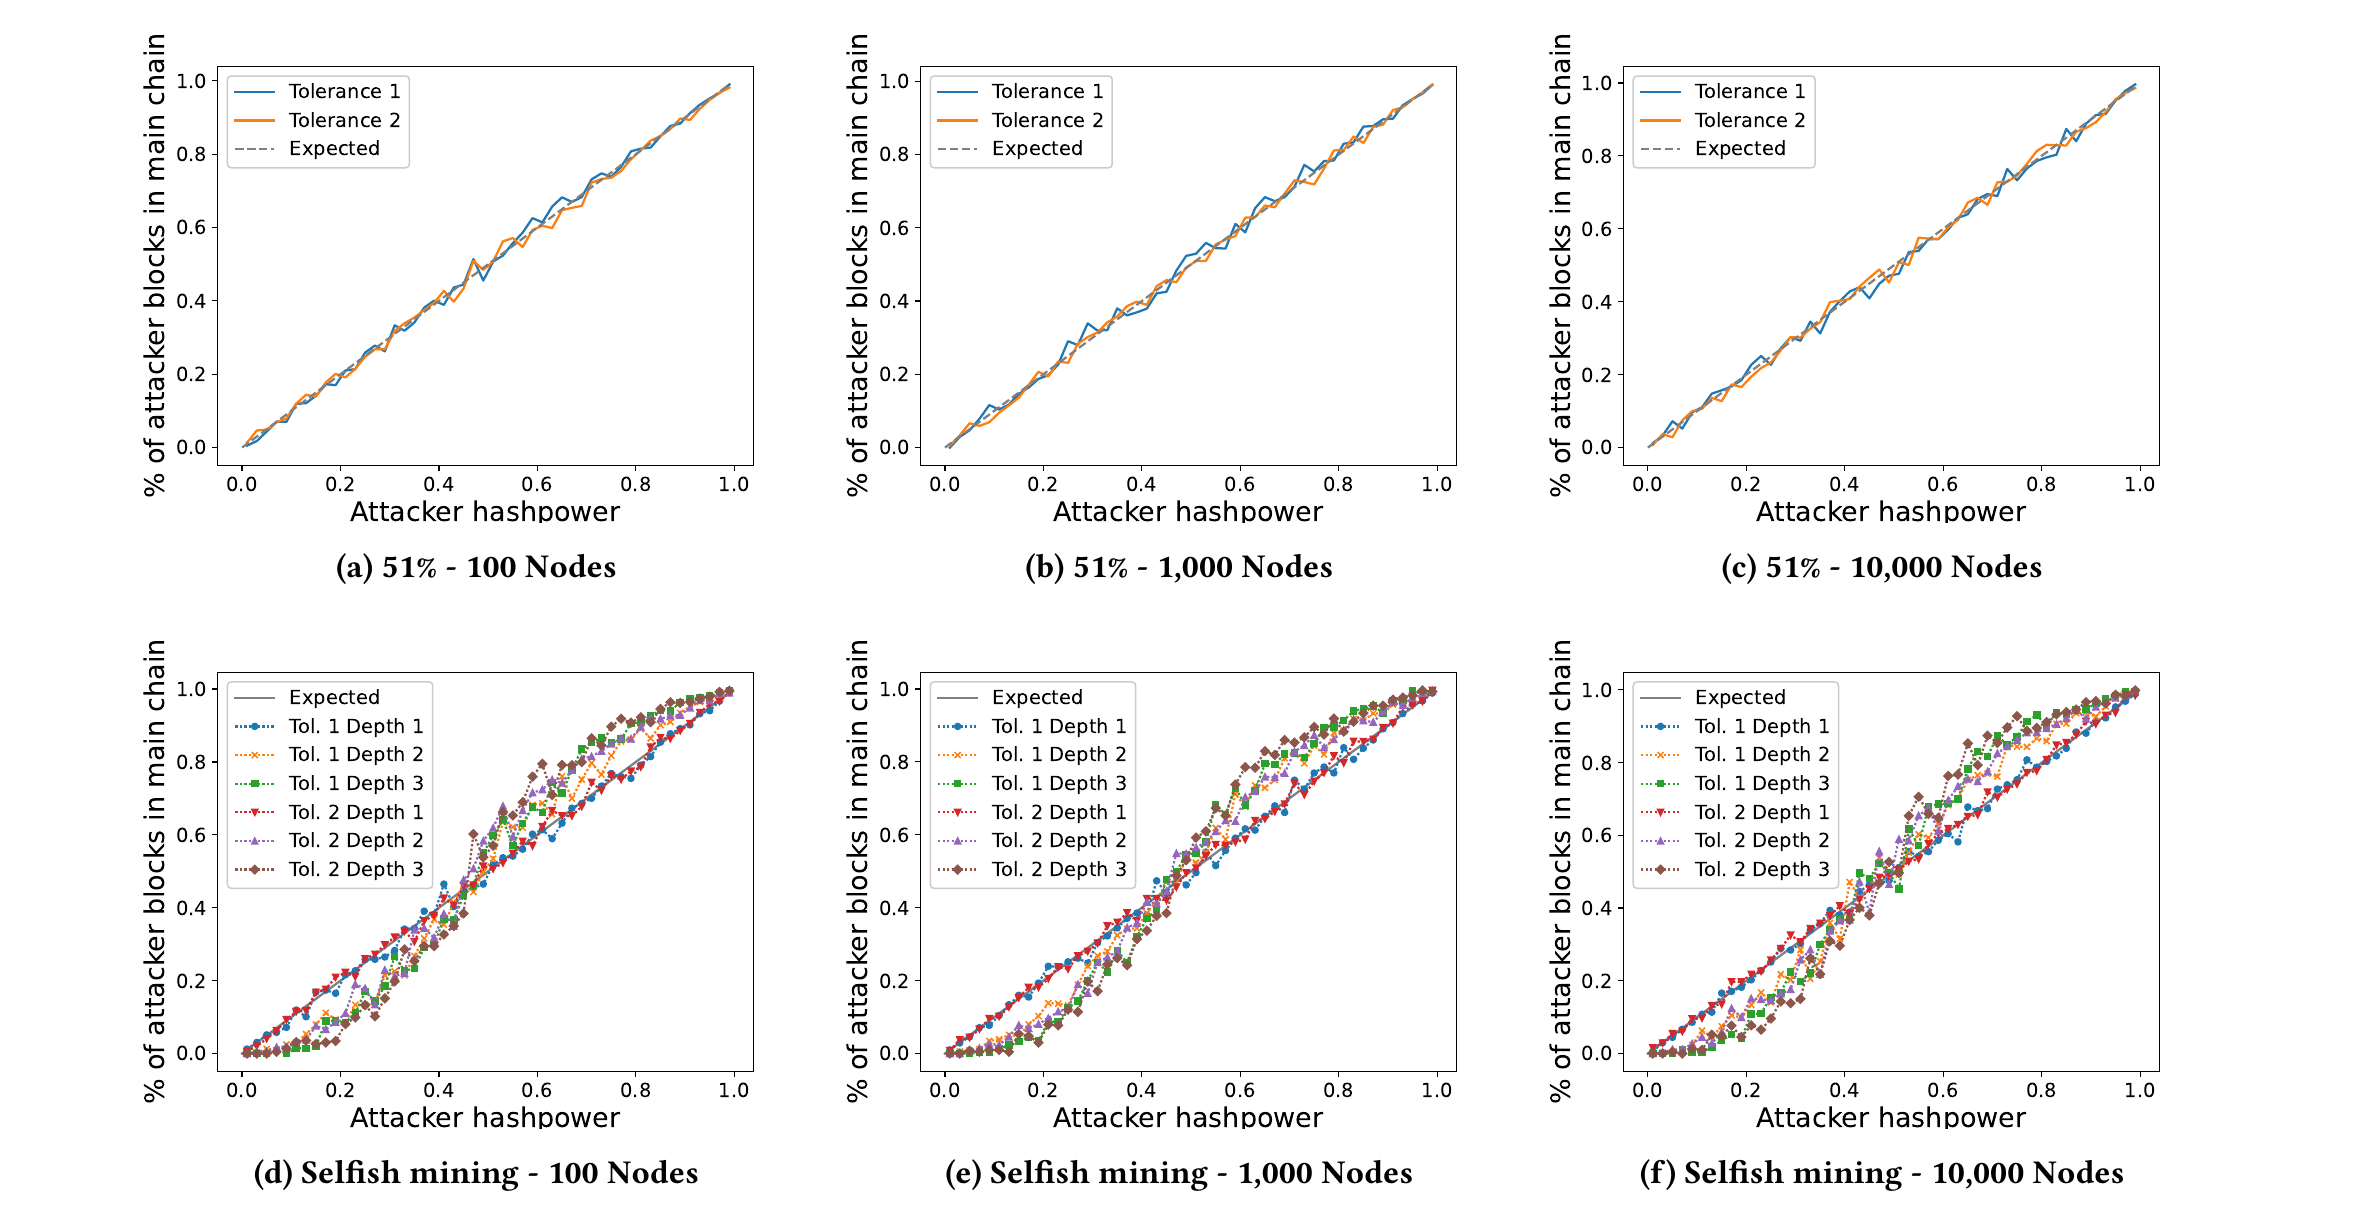
\includegraphics[width=0.90\textwidth]{figures/paper_original/figure4_hi.png}

  \par\vspace{0.4em}
  {\small\textbf{Reproducción}\par}
  \vspace{0.2em}
  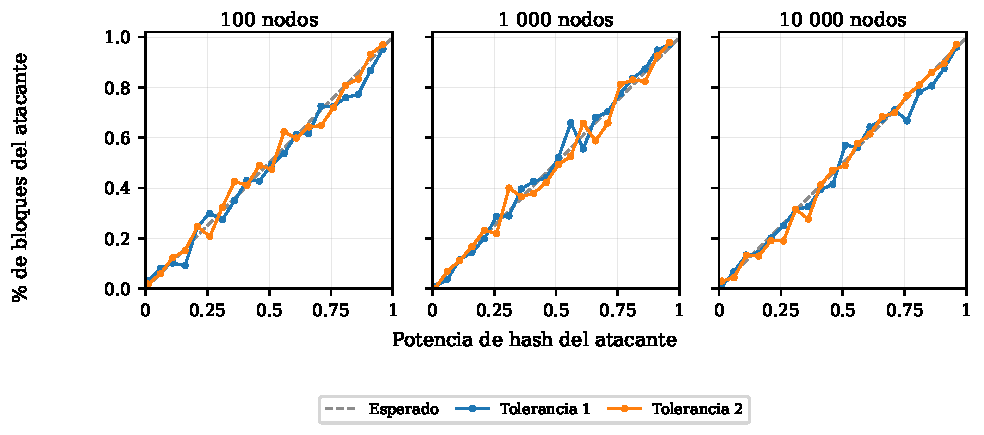
\includegraphics[width=0.90\textwidth]{figures/fig_51.pdf}

  \par\vspace{0.1em}
  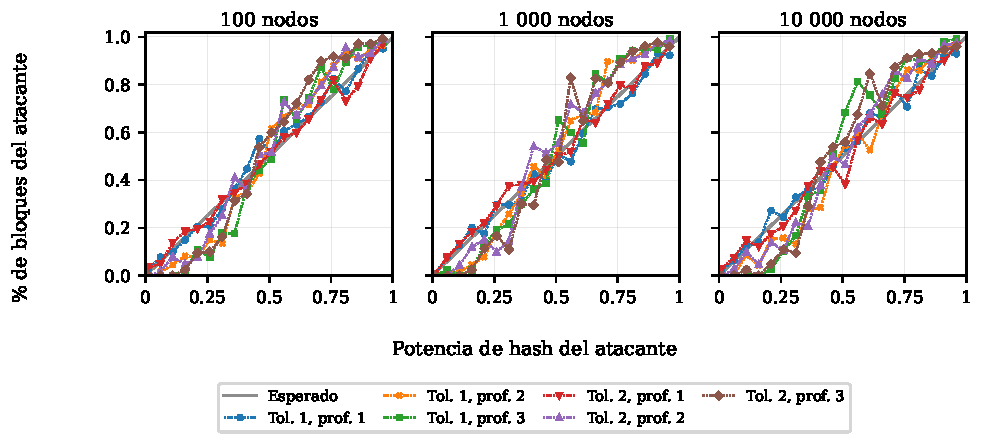
\includegraphics[width=0.90\textwidth]{figures/fig_selfish_committed.pdf}
  \caption{Comparación del ataque del 51\,\% y de los bloques comprometidos por minería egoísta. Arriba: Figura~4 del artículo; abajo: reproducción, con la fila superior para el 51\,\% y la inferior para minería egoísta. Los paneles corresponden a 100, 1\,000 y 10\,000 nodos. La figura original proviene de \cite{pimpini2025rblocksim}.}
  \label{fig:cmp-ataques}
\end{figure}

El ataque del 51\,\% se mantiene cerca de la diagonal en ambas tolerancias (MAE 0.020--0.031). La minería egoísta conserva el abanico de curvas y el efecto de la profundidad: el MAE crece de 0.024--0.032 en profundidad 1 a 0.084--0.103 en profundidad 3.

\begin{figure}[H]
  \centering
  {\small\textbf{Artículo (Figura~6)}\par}
  \vspace{0.2em}
  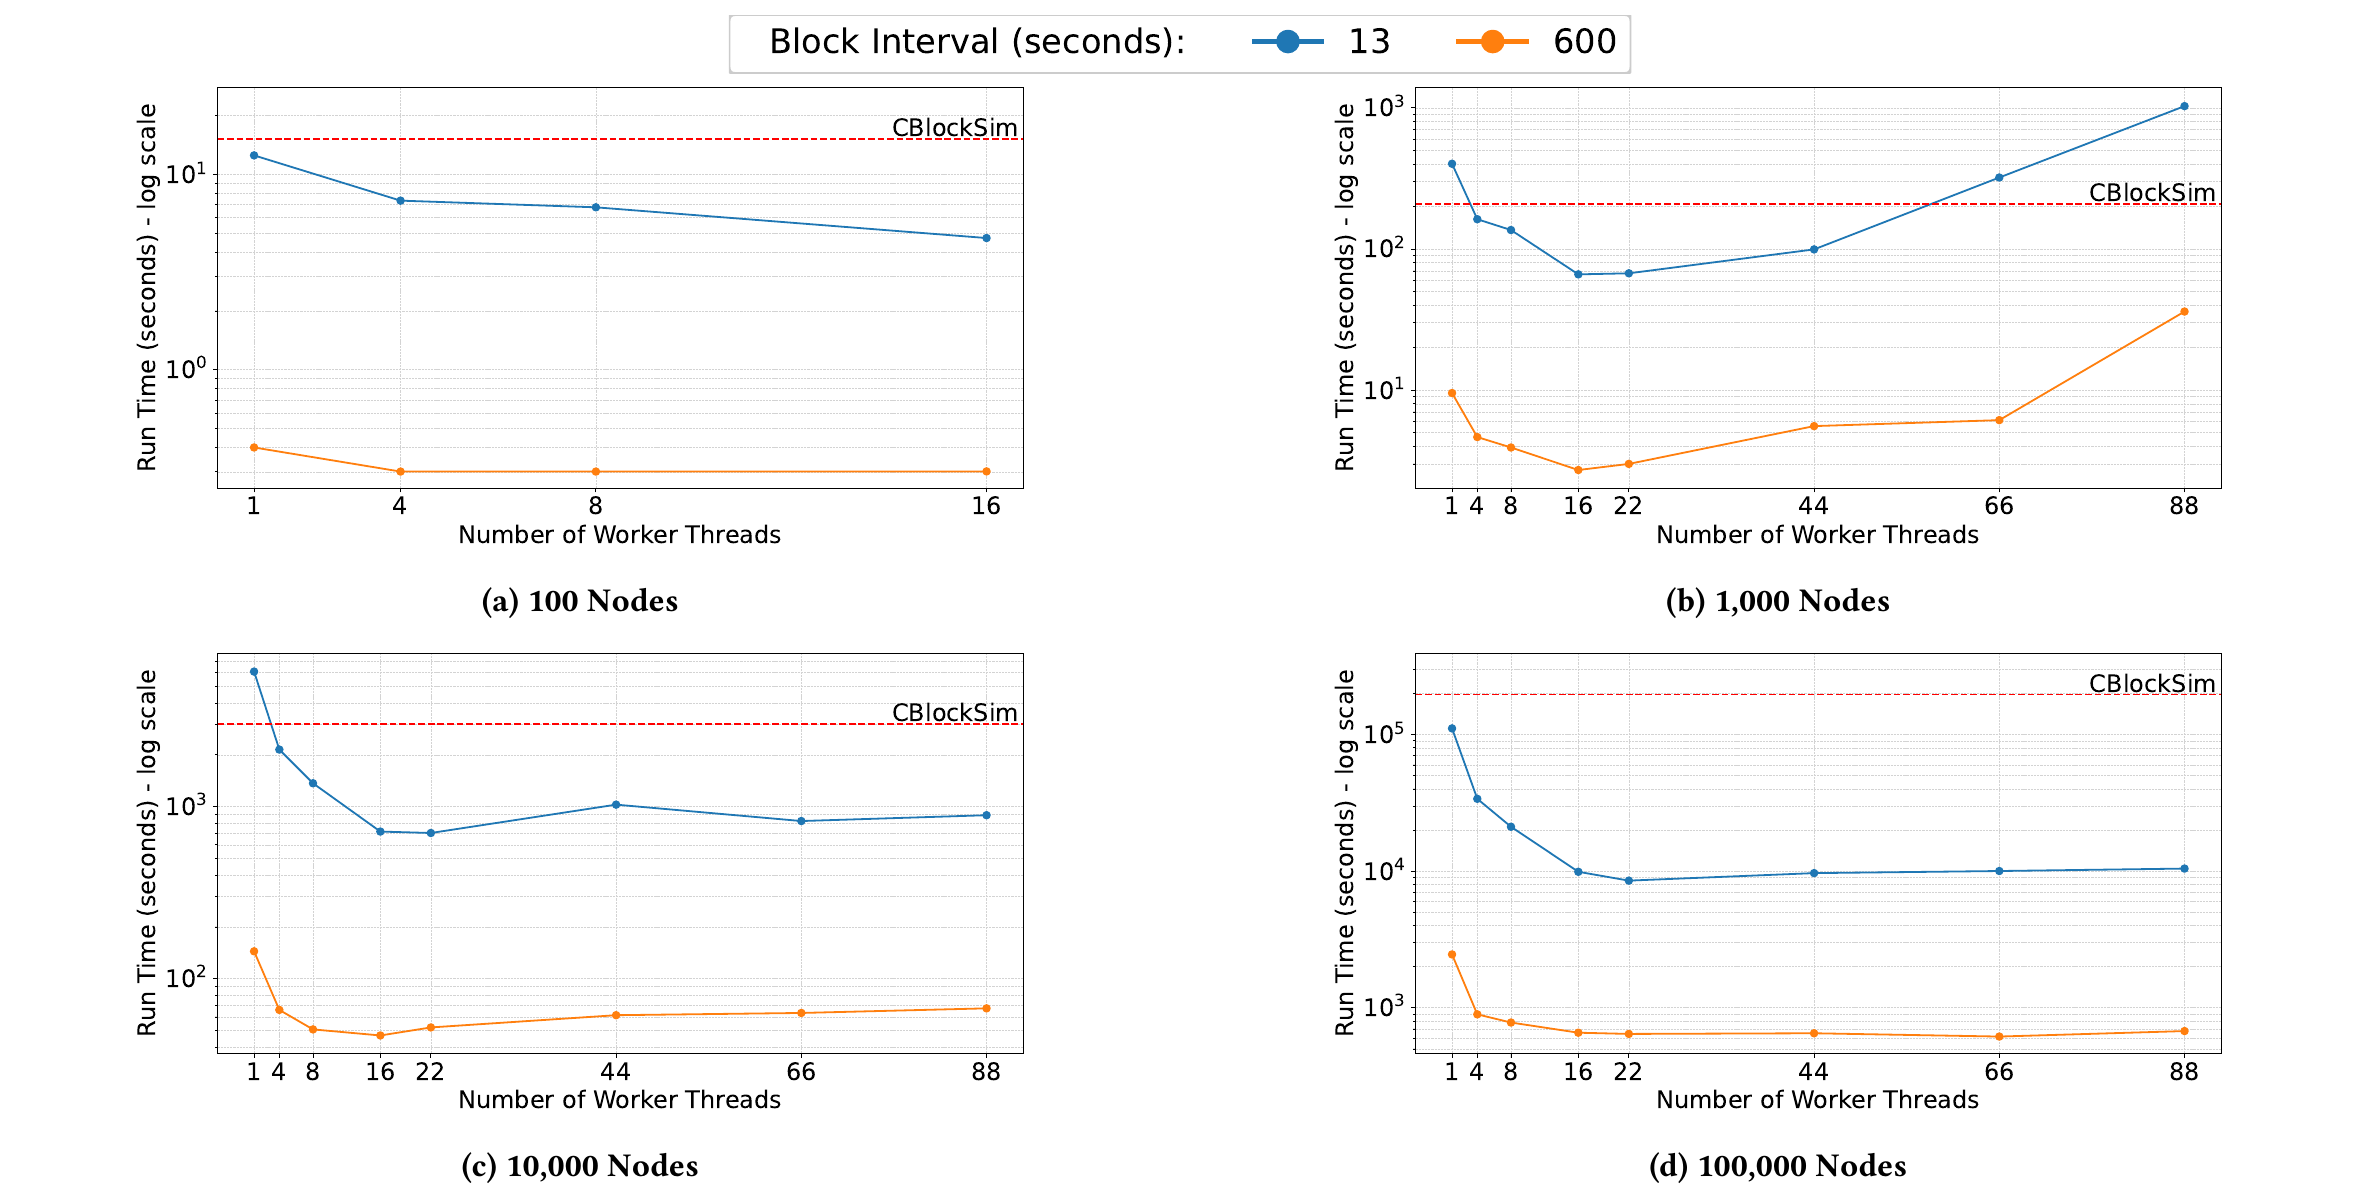
\includegraphics[width=\textwidth]{figures/paper_original/figure6_hi.png}

  \par\vspace{0.45em}
  {\small\textbf{Comparación directa en los hilos comunes}\par}
  \vspace{0.2em}
  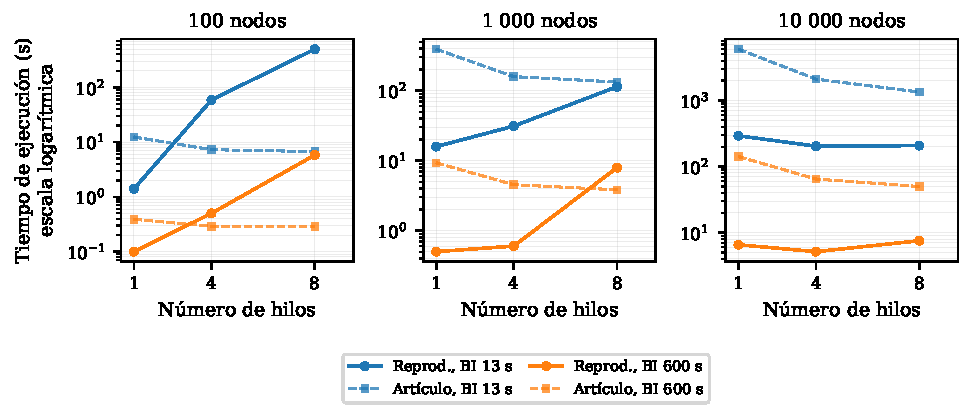
\includegraphics[width=0.92\textwidth]{figures/fig_performance_vs_paper.pdf}
  \caption{Comparación del rendimiento. Arriba: Figura~6 del artículo, que incluye la referencia CBlockSim y el panel de 100\,000 nodos. Abajo: RBlockSim del artículo (líneas discontinuas) frente a la reproducción (líneas continuas) en 1, 4 y 8 hilos. La línea CBlockSim no se reproduce y el panel de 100\,000 no tiene equivalente directo.}
  \label{fig:cmp-rendimiento}
\end{figure}

El artículo sitúa el máximo de rendimiento en 16--22 hilos y muestra una mejora en todas las redes. La reproducción solo cubre 1, 4 y 8 hilos: en 100 y 1\,000 nodos el tiempo se degrada, mientras que en 10\,000 y 50\,000 mejora hasta $2.02\times$. La diferencia se explica por el límite de 12 vCPU, el hardware distinto y la ausencia de repeticiones.

\begin{figure}[H]
  \centering
  \begin{minipage}[t]{0.48\textwidth}
    \centering
    {\small\textbf{Artículo (Figura~7)}\par}
    \vspace{0.2em}
    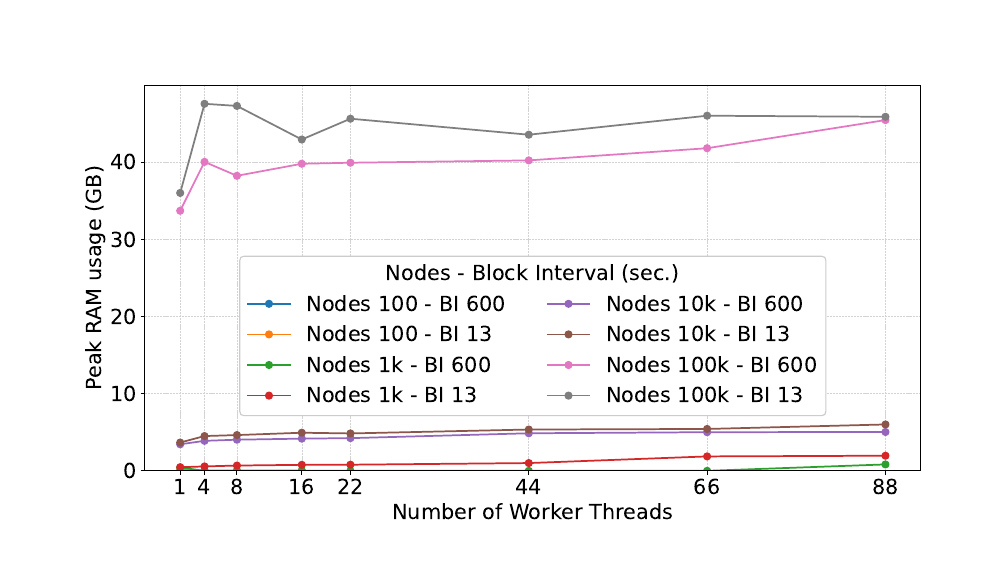
\includegraphics[width=\linewidth]{figures/paper_original/figure7_hi.png}
  \end{minipage}\hfill
  \begin{minipage}[t]{0.48\textwidth}
    \centering
    {\small\textbf{Reproducción}\par}
    \vspace{0.2em}
    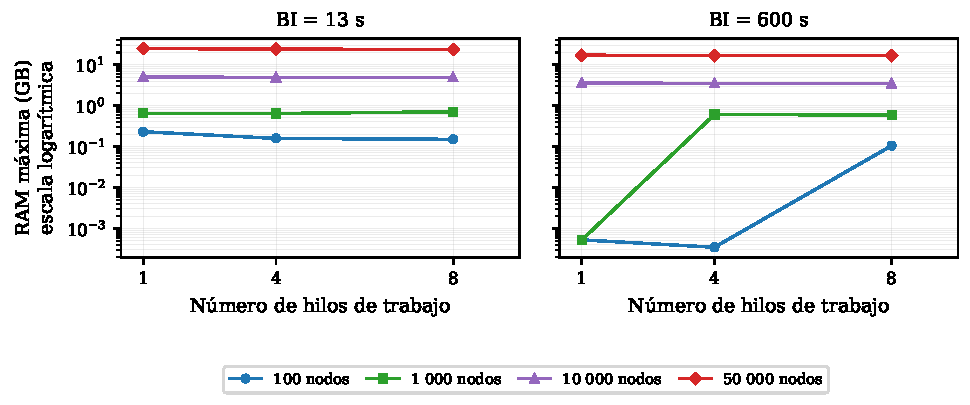
\includegraphics[width=\linewidth]{figures/fig_ram.pdf}
  \end{minipage}

  \par\vspace{0.6em}
  \begin{minipage}[t]{0.48\textwidth}
    \centering
    {\small\textbf{Artículo (Figura~8)}\par}
    \vspace{0.2em}
    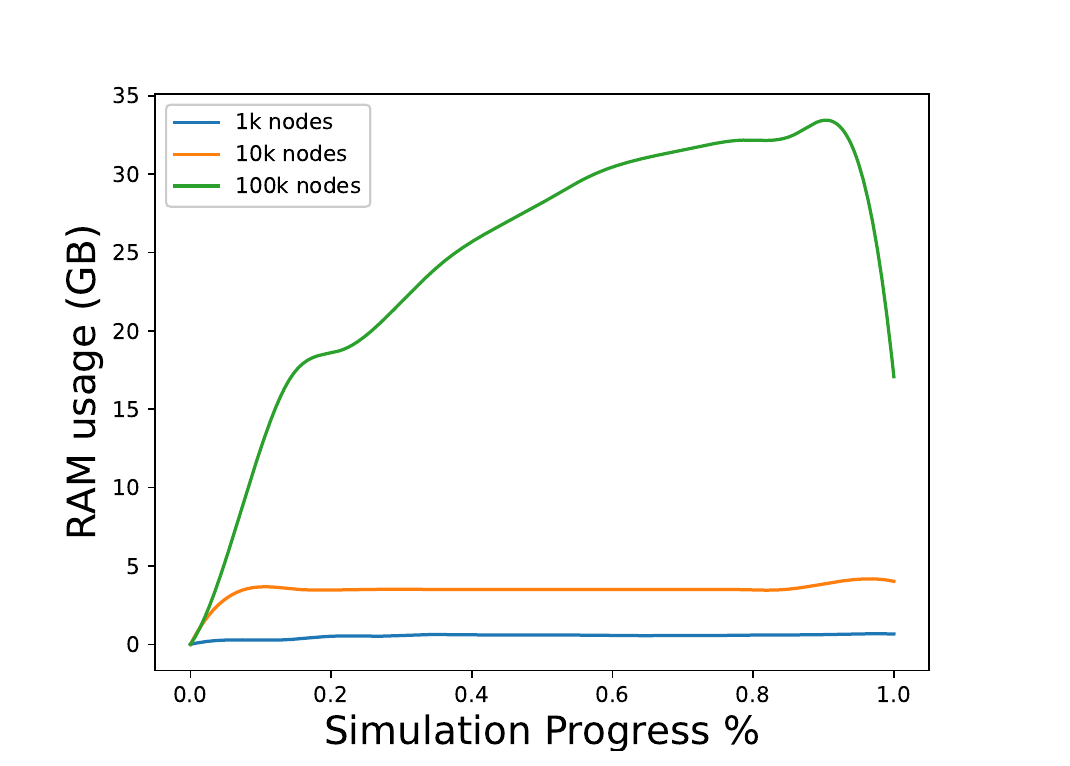
\includegraphics[width=\linewidth]{figures/paper_original/figure8_hi.png}
  \end{minipage}\hfill
  \begin{minipage}[t]{0.48\textwidth}
    \centering
    {\small\textbf{Reproducción}\par}
    \vspace{0.2em}
    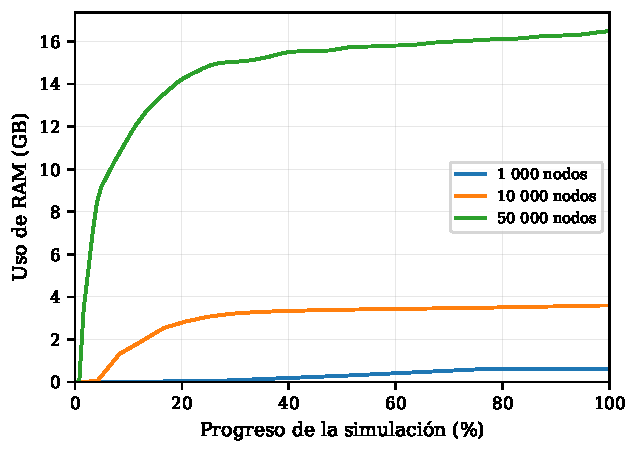
\includegraphics[width=\linewidth]{figures/fig_ram_history.pdf}
  \end{minipage}
  \caption{Comparación del uso de memoria. Arriba: pico de RAM (Figura~7 del artículo frente a la reproducción). Abajo: evolución agregada (Figura~8 del artículo frente a la reproducción). El artículo reporta 100\,000 nodos; la reproducción, 50\,000. La caída final de la curva del artículo corresponde al cierre de la simulación; la reproducción recorta ese tramo para comparar la meseta.}
  \label{fig:cmp-memoria}
\end{figure}

La memoria máxima y la evolución agregada conservan la forma y el orden de magnitud. Para 10\,000 nodos la reproducción obtiene 3.5--5.0\,GB, dentro del rango aproximado de 3.4--5.9\,GB del artículo; para 50\,000 obtiene 16.6--24.9\,GB, consistente con los 35--47\,GB que el artículo reporta para 100\,000. La comparación con la red de 100\,000 es indirecta.

\subsection{Síntesis de la comparación}

La Tabla~\ref{tab:resumen} sintetiza el estado de cada figura. La reproducibilidad funcional es alta: la validación estadística y los ataques mantienen las tendencias y los órdenes de magnitud del artículo. La reproducibilidad de rendimiento es parcial porque no se pudo verificar el máximo de 16--22 hilos ni ejecutar la red de 100\,000 nodos. La memoria es consistente en orden de magnitud. Las diferencias de rendimiento no implican un fallo del artículo: se explican por el entorno de ejecución, el número de iteraciones y posibles diferencias de configuración no registradas.

\begin{table}[htbp]
\caption{Resumen del estado de reproducción de las figuras del artículo.}
\label{tab:resumen}
\centering
\small
\renewcommand{\arraystretch}{1.12}
\begin{tabularx}{\textwidth}{l>{\raggedright\arraybackslash}X>{\raggedright\arraybackslash}Xl}
\toprule
\rowcolor{tablehead}
\textcolor{white}{\textbf{Figura}} &
\textcolor{white}{\textbf{Artículo}} &
\textcolor{white}{\textbf{Reproducción}} &
\textcolor{white}{\textbf{Estado}} \\
\midrule
3 & Tasa de minería proporcional a la potencia de hash & $R^2 \ge 0.9969$, MAE $\le 0.0127$ & Conforme \\
4a--4c & El 51\,\% sigue la diagonal & MAE 0.020--0.031 & Conforme \\
4d--4f & Minería egoísta; profundidad 3 compromete menos & Tendencias equivalentes & Conforme (cualitativo) \\
5 & El éxito crece con $h$ y se satura & Curvas equivalentes, más irregulares & Conforme (cualitativo) \\
6 & Pico de rendimiento en 16--22 hilos & Solo 1, 4 y 8 hilos; sin pico verificable & Parcial / no verificable \\
7 & 10k: 3.4--5.9\,GB; 100k: 35--47\,GB & 10k: 3.5--5.0\,GB; 50k: 16.6--24.9\,GB & Conforme en orden de magnitud \\
8 & 1k: $\sim$1\,GB; 10k: 8--9\,GB; 100k: $\sim$35\,GB & 1k: 0.6\,GB; 10k: 3.6\,GB; 50k: 16.6\,GB & Parcial \\
\bottomrule
\end{tabularx}
\end{table}

\subsection{Limitaciones}

\begin{itemize}[leftmargin=1.2em, itemsep=2pt, topsep=3pt]
  \item \textbf{Límite de núcleos.} La máquina dispone de 12 vCPU; las ejecuciones con 16 o más hilos fallaron. No fue posible verificar el pico de rendimiento en 16--22 hilos ni la degradación posterior.
  \item \textbf{Una sola iteración.} El artículo promedia cinco ejecuciones; aquí se ejecutó una por configuración. Esto aumenta la varianza de las curvas de ataque y de los tiempos.
  \item \textbf{Red máxima reducida.} La red de 100\,000 nodos se sustituyó por 50\,000 nodos, por lo que la comparación con las Figuras~6d y~8 es indirecta.
  \item \textbf{Hardware y configuración.} El procesador y la memoria difieren del servidor del artículo. Además, el artefacto no registra en los metadatos la topología efectiva ni el fanout, lo que impide atribuir con certeza las diferencias de rendimiento.
  \item \textbf{Valores del artículo digitalizados.} Los valores de las Figuras~6 y~7 del artículo se obtuvieron por digitalización visual del PDF y se usan solo como referencia aproximada.
\end{itemize}

%============================================================
%  5. CONCLUSIONES
%============================================================
\section{Conclusiones}
\label{sec:conclusiones}

\begin{enumerate}[leftmargin=1.4em, itemsep=3pt, topsep=4pt]
  \item \textbf{La validación estadística se reproduce con alta fidelidad.} La tasa de minería sigue la esperada con $R^2 \ge 0.9969$ y MAE $\le 0.0127$ en las tres redes. El modelo de Proof of Work basado en una distribución exponencial es estadísticamente correcto.
  \item \textbf{Los ataques se reproducen cualitativamente.} El ataque del 51\,\% sigue la diagonal y no muestra una aceptación desproporcionada. La minería egoísta presenta el crecimiento y la saturación esperados; la profundidad 3 reduce el porcentaje de bloques comprometidos en potencias bajas y medias.
  \item \textbf{El rendimiento se reproduce solo parcialmente.} En 100 y 1\,000 nodos la paralelización degrada el tiempo; en 10\,000 y 50\,000 nodos mejora de forma moderada (hasta $2.02\times$). El pico en 16--22 hilos no pudo verificarse por el límite de 12 vCPU.
  \item \textbf{La memoria es consistente en orden de magnitud.} Los 10\,000 nodos requieren 3.5--5.0\,GB y los 50\,000 nodos 16.6--24.9\,GB. La forma de las curvas reproducidas (Figura~\ref{fig:ram_history}) coincide con la de la Figura~8 del artículo, con valores absolutos menores.
\end{enumerate}

En conjunto, RBlockSim es funcionalmente reproducible y estadísticamente sólido. Sus resultados de ataques y memoria son razonables; el rendimiento es la parte más sensible al entorno y requiere hardware adecuado, repeticiones y un registro completo de la configuración.

%============================================================
%  REFERENCIAS
%============================================================
\vspace{1em}
\printbibliography[title={Referencias}]

\end{document}
